%\pdfoutput=1
%\input{style.tex}
\documentclass[letterpaper,useAMS,usenatbib]{mn2e}
\usepackage[colorlinks=true,
            linkcolor=blue,
            urlcolor=blue,
					  citecolor=blue]{hyperref}
\usepackage{amssymb}
\usepackage{graphicx}
\usepackage{amsmath}
\usepackage[amssymb]{SIunits} 
\usepackage{booktabs}
\usepackage{hhline}
\usepackage{breqn}
\usepackage{standalone}
\usepackage{dcolumn}
	\newcolumntype{d}[1]{D{.}{.}{#1}}
\usepackage{tabularx}
\usepackage{booktabs}
\usepackage{microtype}
\usepackage{algpseudocode}
\usepackage[]{algorithm2e}
\graphicspath{{figures/}}
\newcommand{\mc}[1]{\multicolumn{1}{c}{#1}} % handy shortcut macro
%-----------------------------------------------------------------------
\def\apjl{ApJL }
\def\aj{AJ }
\def\apj{ApJ }
\def\pasp{PASP }
\def\spie{SPIE }
\def\apjs{ApJS }
\def\araa{ARAA }
\def\aap{A\&A }
\def\nat{Nature }
\def\mnras{MNRAS }
\def\mnrasl{MNRASL }
\providecommand{\eprint}[1]{\href{http://arxiv.org/abs/#1}{#1}}
\providecommand{\adsurl}[1]{\href{#1}{ADS}}
\providecommand{\ISBN}[1]{\href{http://cosmologist.info/ISBN/#1}{ISBN: #1}} 
%-----------------------------------------------------------------------
\title[
	Galaxy-dark matter offsets in galaxy clusters and groups of the
Illustris simulation
]
{Galaxy-dark matter offsets in galaxy clusters and groups of the
Illustris simulation}
\author[Karen Y. Ng et al.]{Karen Y. Ng,$^{1}$
	Annalisa P. Pillepich,$^{2}$ 
	William A. Dawson,$^{3}$ 
	D. Wittman,$^{1}$
	\newauthor Lars Hernquist,$^{2}$
	etc. [order TBD]
}
\begin{document}
\date{arXiv} \pagerange{\pageref{firstpage}--\pageref{lastpage}}
\pubyear{2015} \maketitle\label{firstpage}
\begin{abstract} 
	Being able to find the center of the dark matter component of a galaxy cluster or
	group enables correct stacking and mass estimation if any parametric halo
	profile is employed. 
\end{abstract}
\begin{keywords}
	galaxy clusters, dark matter, something else 
\end{keywords}
\section{INTRODUCTION} 

Galaxies that belongs to a galaxy cluster or group are stochastic samples
of the underlying dark matter mass density. 

We look for summary statistic that would have the least biased estimate of
the dark matter density peak. For stacking the different sets of data, 
find a good proxy for the dark matter density peak is important for the
peak not to be smoothed out. 


\section{DATA}
\subsection{Test data from Gaussian mixture(s)}
In order to examine the performance of commonly used point-estimates of the
distribution of the galaxy data, we test them on Gaussian mixtures with
known mean and variance. \\
Fig 1. one Normal mixture \\  
Fig 2. one big normal mixture and one smaller normal mixture \\ 
Fig 3. bridged normal mixtures \\  

We provide all the code and data of these test in our Bitbucket repository
for comparison purposes for point estimator not listed.

\subsection{Data from the Illustris simulation} 
\begin{figure}
	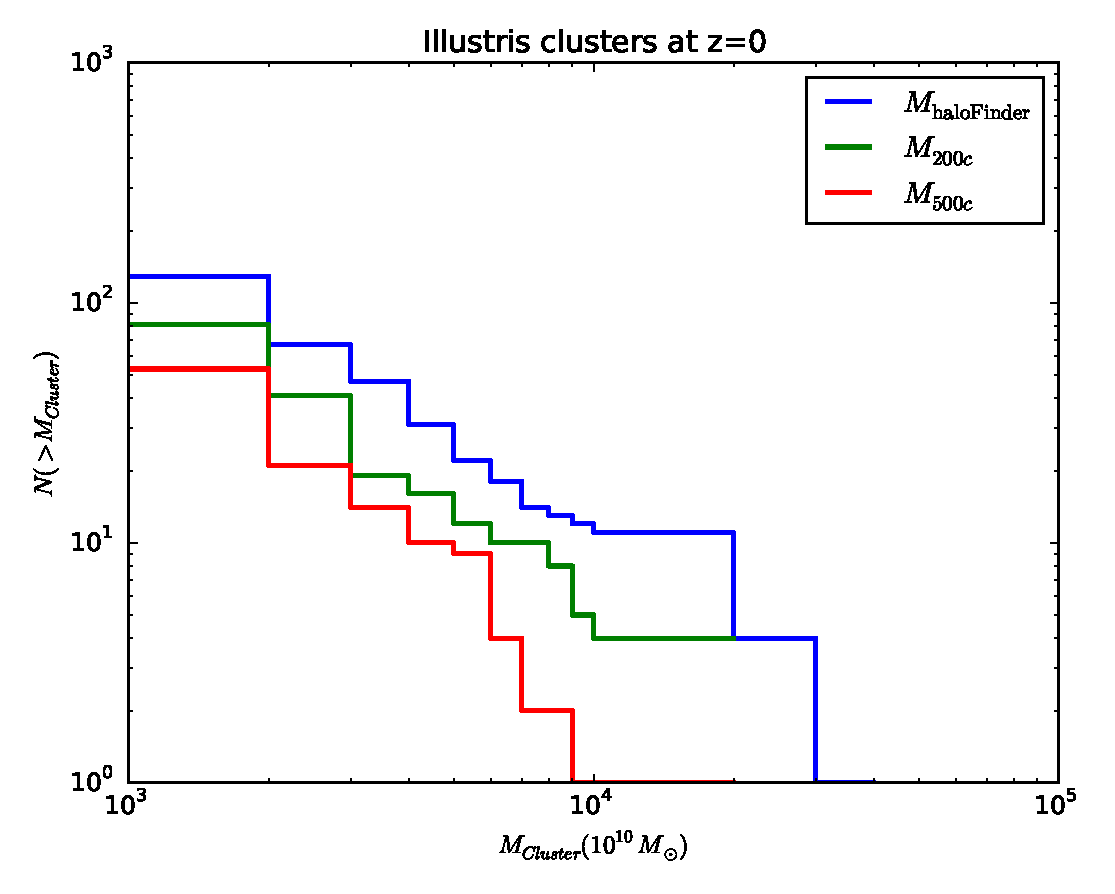
\includegraphics[width=.95\linewidth]{clusterMassDist.eps}
	\caption{
		\label{fig:config}}
\end{figure}


\subsubsection{Properties of the galaxy clusters / groups}
Most important properties of the galaxy clusters that we examine in this
study include, colors, magnitude, richness, concentration and non-relaxedness. We define
and examined these properties one by one. 
Fig 4. Relaxedness 
Fig 5. 

Richness characterizes the number of galaxies in a given cluster.
We provide several definitions of non-relaxedness to characterize whether
the clusters underwent any recent merger activities. These definitions of
non-relaxedness.
The Shapiro-Wilk statistic can characterize the deviation from normality
with the highest statistical power ().


\subsubsection{Volume Selection}
1. Rockstar halo finder 
2. Light cone 
3. spatial projections 
\subsubsection{Galaxy Selection}
\subsubsection{Galaxy weights}
\subsubsection{Data with and without noise}
1. Mass-richness diagram - with different cuts  
\section{METHODS} 
\subsection{Galaxy Centers}
\subsubsection{Unweighted and weighted centroids}
We follow the usual definition of spatial centroid as 
\begin{equation}
	\vec{x} = \frac{1}{n} \sum_i \vec{x}_i. 
\end{equation}
While the weighted centroids are just: 
\begin{equation}
	\vec{x}_w = \frac{\sum_i w_i \vec{x}_i}{\sum_i w_i},
\end{equation}
for each spatial dimension and the weights $w_i$ for the $i-th$ galaxy
is described in section.
Centroids and weighted centroids can be biased by merging activities yet do
not provide explicit evidence for ongoing merger or accretion. 



\subsubsection{Cross-validated Kernel Density Estimation (KDE) and the peak finder} 
We employed a KDE algorithm to infer a smooth density distribution of the
galaxies while using smoothed cross-validation to obtain the optimal smoothing
bandwidth matrices ($H$). Specifically, we made use of the KDE function in
the statistical package ks (Duong) in the R statistical computing environment (R Core Team 2014).
Cross validation eliminates free parameters in the KDE and minimizes
the asymptotic mean-integrated squared error (AMISE) for a best fit to the
data.
After obtaining the KDE estimate, we employed a finite differencing algorithm
to find the local maxima. We sorted the local maxima according to the KDE
density at the maxima locations and identified the dominant peak. 

\subsubsection{Shrinking aperture}
Another method that is popular among astronomers for summarizing a spatial
distribution include what we call a shrinking aperture method.
We test if the shrinking aperture method is able to recover the highest peak reliably.
This method is dependent on the initial location of the aperture.
Furthermore, the convergence criteria is not set objectively.
\begin{algorithm}
	\caption{Shrinking aperture algorithm}
	\KwData{subhalo that satisfy cuts as a galaxy}
	 \hrulefill

	initial_center = mean(data\_array)\\
 	dist\_array = euclidean_dist(initial_center, data_array)\\
 	apert = get\_90th\_percentile(dist\_array)\\ 
	\While{ (newCenterDist - oldCenterDist) / oldCenterDist $\geq$ 2e-2}{
 		new data array = old data array within apert\\
 		newCenter = mean value of new data along each spatial dimension 
	}   \hrulefill
 \end{algorithm}


\subsubsection{Brightest Cluster Galaxies (BCG)}
From the provided 


\subsection{DM Centers}
\subsection{Finding offsets} 

We computed the projected offsets between the galaxy density peaks inferred from the
cross-validated KDE and the dark matter density peak. (TBD) 
The viewing angles of the projections are defined by an elevation angle
$\xi$ and an azimuthal angle $\phi$. 
We sample at 5 evenly spaced values of $\xi$ where $0 \leq \xi \leq \pi / 2$ and 
10 evenly spaced values of $\phi$ where $0 \leq \phi \leq \pi$, to give 50
samples for each cluster with mass $> 10^{14} M_\sun$. 

This method gives us samples of the joint distribution: 
\begin{equation}
	P(\Delta \eta, \phi, \xi, h_{mer}, \psi_g, \psi_D, I_g, I_D | \theta,
	\sigma_{CDM}). 
\end{equation}


Binning the samples based on $\Delta \eta$ and $h_{mer}$ only gives us the
marginal distribution:
\begin{equation}
	P(\Delta \eta, h_{mer} | \theta, \sigma_{CDM}),
\end{equation}
that we have far too few samples of \dots


\section{RESULTS} 
\subsection{Benchmark results from Gaussian mixtures} 
(We expect some of the existing point-estimates are quite crappy e.g. the
shrinking aperture method, and will not
use them for the Illustris data) 

\subsection{Galaxy-DM Offset in Illustris}
\subsubsection{Projected offsets}
\subsubsection{Correlations between the offsets and properties of the cluster / groups}
\section{DISCUSSION}
\subsection{Comparison to other simulations}
\subsection{Comparison to other observational studies}
\subsection{Galaxy-DM Offset in Merging Galaxy Clusters}
\section{ACKNOWLEDGEMENTS}
% K. Ng would like to thank D. Hogg for useful discussion on 
% alternative ways of characterizing differences between DM and galaxy
% distributions.

\bibliographystyle{mn2e}
\bibliography{galDMoffset.bib}
\bibliography{R_package.bib}
\appendix
\section{KDE}
\clearpage\bsp\label{lastpage} 
\end{document}
